\chapter{Introdução: O que é a Termodinâmica Clássica?}
\label{chap:introduction}

    Para começar, o que é a Termodinâmica? Uma resposta possível pode ser
    obtida da literatura:
    \enquote{%
        é um ramo da ciência fundamental e aplicada
        que descreve de forma macroscópica as forças motrizes que estabelecem
        os fluxos de energia (na forma de trabalho e calor) e as condições para
        o equilíbrio dentro de um sistema (região arbitrária no espaço).
        Entende-se por equilíbrio um estado do sistema onde estas forças
        motrizes estão ausentes ou inoperantes e o referido sistema não possui
        mais a capacidade de se alterar espontaneamente.%
    }

    Parece muito complicado, não?

    \section{Uma Definição para Substância Pura e Sistema}

    Vamos tentar construir aos poucos uma definição mais acessível, embora
    talvez menos abrangente. Para isso, precisamos estabelecer um vocabulário
    comum fundamentado em uma série de conceitos.

    Substância pura é aquela porção de matéria de composição química definida e
    que mantém a sua composição mesmo sob mudança de fase (água pura na forma
    de sólido, liquido ou vapor não deixa de ser água...).

    O sistema termodinâmico será para nós qualquer região delimitada no espaço
    que, ou contém uma ou mais substâncias puras, ou é composto de subsistemas
    que por sua vez são sistemas termodinâmicos (claramente uma definição
    recursiva de sistema...).

    Além disso, tudo o que não pertence ao sistema é a sua vizinhança e
    exatamente na interface entre o sistema e a sua vizinhança, existe uma
    região imaginária sem massa nem espessura extremamente importante chamada
    fronteira do sistema. Observe-se com atenção que tanto a vizinhança como a
    fronteira são ambos determinados relativamente ao sistema escolhido.


    \section{Que Tal um Exemplo?}

    Vejamos então um exemplo: Seja um cilindro de aço (uma liga metálica) de
    paredes com determinada espessura contendo gás natural (uma mistura de
    substâncias puras). Poderemos, de acordo com a nossa definição, estabelecer
    um sistema termodinâmico como sendo a porção de gás natural encerrada no
    cilindro. Neste caso, a vizinhança será tudo o mais além daquele volume de
    gás --- as paredes do cilindro, o ambiente externo ao cilindro, etc. A
    fronteira do sistema estará delimitada pela interface entre o volume de gás
    e a parede interna do cilindro. Por outro lado, o nosso sistema poderia ser
    o gás mais o cilindro. Permaneceríamos ainda dentro de nossa definição,
    pois este seria composto de uma mistura de gases e de uma liga metálica.
    Neste caso, a fronteira do sistema estaria entre a parede externa do
    cilindro e o ambiente exterior, que neste caso se confunde com a vizinhança
    do sistema.  Sob esta escolha, o sistema poderá ser dividido em dois
    subsistemas: a porção de gás e o cilindro sólido, cada um deles composto de
    uma mistura de substâncias puras. A propósito, lembre-se sempre que o
    subsistema é também um sistema de pleno direito e, portanto, dotado de sua
    própria vizinhança e respectiva fronteira!

    Acredite, a indefinição na escolha do sistema é, provavelmente, um dos
    maiores responsáveis pelos erros cometidos na interpretação e solução de
    problemas em termodinâmica...


    \section{Estado e Propriedades}

    Pois bem, a nossa definição especializada de sistema tem um propósito,
    analisar o estado termodinâmico.  O estado  termodinâmico (de equilíbrio)
    do sistema termodinâmico é caracterizado através do valor
    \enquote{instantâneo} de suas propriedades termodinâmicas (o
    \enquote{retrato} de suas propriedades). Mas o que são as tais propriedades
    termodinâmicas?

    Propriedades termodinâmicas são aquelas propriedades do sistema cujo valor
    presente não depende dos valores passados ou futuros, ou seja, da história
    da evolução do sistema, ou da sucessão de estados do sistema, ou ainda em
    outras palavras, do processo termodinâmico pelo qual passou o sistema para
    chegar naquele estado presente (pode-se dizer: a propriedade simplesmente
    é...).

    As propriedades termodinâmicas podem ser extensivas, quando dependem
    linearmente da massa do sistema, como é caso do volume (dividindo-se a
    massa por uma proporção, o volume divide-se na mesma proporção) e
    intensivas, cujo valor não se altera com a alteração da massa, como a
    temperatura, a pressão e a densidade (massa específica) do sistema, que
    permanecem as mesmas, não importa a proporção de massa do sistema que
    selecionemos. Todas as propriedades extensivas podem ser divididas pela
    massa, criando-se dessa forma uma nova propriedade intensiva
    correspondente. Se dividirmos o volume - propriedade extensiva - do sistema
    pela sua massa, obteremos o volume específico, propriedade intensiva, ou
    para distinguir das propriedades intensivas próprias, chamaremos aqui de
    intensiva associada ou \enquote{intensivada}. Podemos citar, então, a
    temperatura T e a pressão absolutas P como propriedades intensivas próprias
    e o volume V e a própria massa m como propriedades extensivas.
    Encontraremos ainda muitas outras propriedades extensivas e intensivas ao
    longo do nosso estudo, mas todas elas têm as mesmas características.

    Um processo termodinâmico é qualquer alteração do estado do sistema. Se
    apenas uma (das, por enquanto inumeráveis) propriedades termodinâmicas do
    sistema sofrer uma alteração infinitesimal, o estado também será alterado
    infinitesimalmente e diz-se que o sistema terá sido submetido a um processo
    infinitesimal. Se a mudança de estado for discreta, dizemos então que o
    sistema sofreu um processo discreto. Ambos os tipos de processo,
    infinitesimal e discreto serão importantes no nosso estudo.

    \section{Trabalho, Calor e Fluxo de Massa}

    Está claro então que as propriedades são definidas internamente ao sistema.
    Mas como podem seus valores sofrerem alteração? De um modo geral através de
    interações na fronteira do sistema, como representado na
    \cref{fig:thermodynamicSystemInteractions}. Durante um intervalo de tempo
    dt  existem duas espécies de interações do sistema com a sua vizinhança
    através da fronteira: as interações de energia, através de transferência de
    trabalho mecânico (\idiff{\gls{workTransfer}}) e de  transferência de calor
    (\idiff{\gls{heatTransfer}}), que são duas formas distintas de transporte
    de energia; e interação de massa, através de transferência de massa
    (\idiff{\gls{mass}}) através de qualquer parte da fronteira.

    \begin{figure}[!htb]
        \caption{%
            O sistema termodinâmico e suas interações.
        }

        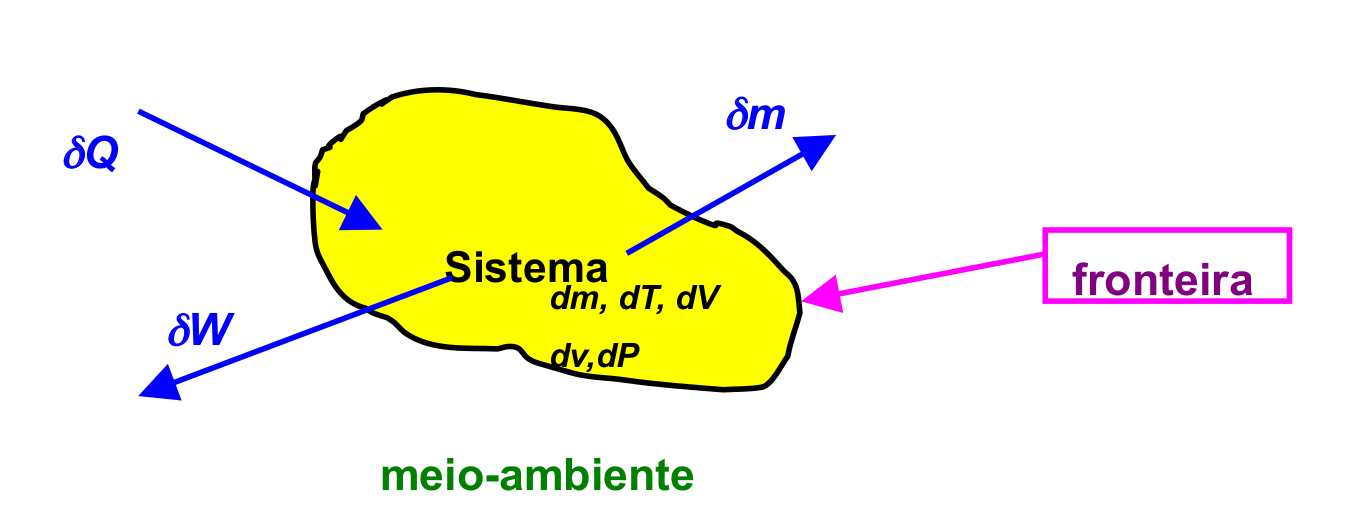
\includegraphics[
            width=0.5\textwidth
        ]   {thermodynamicSystemInteractions.png}

        \label{fig:thermodynamicSystemInteractions}
    \end{figure}

    Mas o que distingue as interações na fronteira do sistema das propriedades
    termodinâmicas? São as três características dessas interações:

    \begin{enumerate}
        \item só são identificadas investigando-se ao longo de toda a fronteira
            do sistema;

        \item só têm existência enquanto o processo (possivelmente
            infinitesimal) ocorre entre dois estados do sistema; e

        \item dependem de cada processo que ocorre entre os mesmos dois
            estados. Esta é razão pela qual adotamos a notação
            \enquote{\idiff{}}, de diferencial não ordinária (cujo valor
            depende do caminho ou processo), para essas grandezas.
    \end{enumerate}

    Entretanto, nunca se esqueça de um importante ponto: se escolhermos um
    outro sistema para representar um aspecto da modelagem do mesmo problema
    real, então todas as interações de trabalho, calor e massa, bem como as
    propriedades termodinâmicas no interior do sistema, deverão ser avaliadas
    relativamente a este novo sistema. O elo de ligação entre os sistemas é
    obviamente a representação da realidade física a partir do qual eles são
    escolhidos.


    \section{O Trabalho Mecânico}

    Sabemos da Mecânica, que a definição de trabalho é
    %
    \begin{equation} \label{eq:0.1}
        \gls{workTransfer}
        =
        -\int{
            \gls{force}
            \dprod
            \diff{\gls{EulerCoord}}
        }
    \end{equation}
    %
    que é a representação matemática do produto interno das forças que atuam
    sobre o corpo pelo deslocamento do ponto de aplicação daquelas mesmas
    forças. Estamos adotando na presente obra a convenção de que o trabalho
    realizado pelo sistema termodinâmico é positivo, daí o sinal negativo na
    Eq. 0.1. Note que esta convenção não é, de forma alguma, universal. Em
    muitas áreas, notadamente a Química, a convenção e exatamente contrária a
    esta.

    Em termodinâmica, podemos dizer para nossos propósitos que o trabalho
    mecânico puro (ou simplesmente trabalho mecânico) é toda aquela interação
    na fronteira cujo efeito sobre a vizinhança puder ser substituído
    unicamente pelo levantamento de um peso. Este, de fato, é o trabalho
    realizado por uma força cujo ponto de aplicação acompanha o movimento.

    No caso de sistemas de potência e refrigeração existem duas únicas formas
    de trabalho mecânico que irão nos interessar. Uma delas é a de deslocamento
    da fronteira \diff{\gls{volume}} em resistência a uma força \gls{forceComp}
    realizada por uma pressão \gls{pressure}, com $\gls{pressure} =
    \dfrac{\gls{forceComp}}{\gls{surfaceArea}}$:
    %
    \begin{equation} \label{eq:0.2}
        \gls{workTransfer}
        =
        \int{
            \gls{pressure}
        }\diff{\gls{specificVolume}}
    \end{equation}
	%
    que é um trabalho positivo para deslocamentos positivos
    ($\diff{\gls{specificVolume}} > 0$) da fronteira, uma vez que a pressão é
    sempre positiva. Podemos afirmar que a força motriz para a transferência de
    trabalho mecânico é o \enquote{gradiente} de pressão. A pressão, por sua
    vez, é uma propriedade termodinâmica intensiva própria do sistema.

    A outra forma de trabalho mecânico importante para nossas aplicações em
    engenharia de energia será o trabalho de cisalhamento na fronteira ou
    trabalho de eixo.

    Um reservatório de pressão (ou reservatório de trabalho) é um sistema
    especial cuja única interação na fronteira é o trabalho mecânico e cuja
    pressão não se altera, qualquer que seja a demanda ou fornecimento de
    trabalho em sua fronteira.

    Um tipo de fronteira de zero-trabalho pode então ser representada por um
    recipiente rígido (isto é, que não sofre deformação alguma sob gradientes
    de pressão), isto é $\diff{\gls{volume}} = 0$, ou com expansão não
    resistida, ou seja, não há um ponto de aplicação de uma força durante a
    expansão, desde que em nenhum dos casos haja trabalhos de eixo.

    Se a restrição sobre o sistema impede qualquer transferência de trabalho
    mecânico, então os processos serão denominados de processos de
    zero-trabalho.


    \section{O Calor}

    Podemos dizer que por exclusão calor é aquela interação de energia na
    fronteira de um sistema que não é trabalho mecânico. Alternativamente,
    calor é a interação de energia que, se não houver restrições, ocorrerá
    entre dois corpos em contato, devido à sua diferença finita de temperatura.
    Uma vez isolados os dois corpos em contato, após um certo tempo, cessará o
    fluxo de calor entre eles. Dizemos então que eles estão em equilíbrio
    térmico entre si. Para que se possa falar em temperatura, é necessário que
    possamos medi-la e compará-la sem ambiguidade. Para isso, lançamos mão de
    um axioma fundamentado na experiência cotidiana, conhecido como Lei Zero da
    Termodinâmica: Se dois corpos estão em equilíbrio térmico com um terceiro,
    então estão em equilíbrio térmico entre si, ou seja, eles estão à mesma
    temperatura.

    A temperatura termodinâmica absoluta, por sua vez, é uma propriedade
    intensiva própria do sistema. É uma grandeza sempre positiva e a força
    motriz para o calor é o potencial ou \enquote{gradiente} de temperatura.

    Talvez as definições de interação de calor, em termos de temperatura, ou de
    trabalho mecânico, a partir da pressão, lhe tenham parecido um tanto quanto
    circulares. De fato, primeiro aprenderemos a distinguir rigorosamente ambas
    as interações de energia entre si quando estudarmos a Segunda Lei da
    Termodinâmica e mais tarde aprenderemos como definir temperatura e pressão
    sem ambiguidades, quando estudarmos as relações que podem ser construídas
    entre as propriedades termodinâmicas.

    Um reservatório térmico (ou reservatório de temperatura) é um sistema
    especial cuja única interação na fronteira é calor e cuja temperatura não
    se altera, qualquer que seja a demanda ou fornecimento de calor através de
    sua fronteira.

    Se em alguma parte da fronteira não houver fluxo de calor através dela,
    então aquela parte é dita adiabática.  Se em toda a fronteira o fluxo de
    calor não é permitido, toda a fronteira será adiabática (isolante perfeito)
    e então todos os processos que ocorrerem sobre o sistema serão
    necessariamente adiabáticos. Uma fronteira adiabática suporta qualquer
    diferença de temperatura entre o sistema e sua vizinhança sem transporte de
    calor, um isolante perfeito. Veja bem, a impossibilidade de transferência
    de calor pela fronteira adiabática não significa que a temperatura no
    interior do sistema não possa se alterar.

    Por outro lado, se a fronteira é permeável a qualquer intensidade de fluxo
    de calor, ela é diatérmica (condutor de calor perfeito), ou seja, a
    fronteira não suporta nenhuma diferença de temperatura entre o sistema e
    sua vizinhança, um condutor perfeito.


    \section{Sistema Fechado, Aberto ou Isolado}

    Se massa não puder atravessar nenhuma parte da fronteira do sistema, ou
    seja, se a fronteira do sistema for impermeável à massa, então o sistema é
    dito fechado. Caso contrário, é denominado sistema aberto ou volume de
    controle. Se a fronteira é permeável a apenas algumas espécies químicas
    então é chamada um tanto inadequadamente de semipermeável.

    Quando nem calor, nem trabalho, nem fluxo de massa são permitidos através
    da fronteira de um sistema, o sistema é dito isolado. Como um caso
    importante, qualquer sistema mais a sua vizinhança compõe um sistema
    isolado (por quê?). A associação do sistema com a sua vizinhança é
    denominada sistema universo.

    No caso de um sistema isolado, claramente os valores das propriedades no
    interior de um sistema isolado só podem ser modificados de um estado de
    equilíbrio por meio de uma evolução espontânea do sistema desse estado até
    alcançar um novo estado de equilíbrio. Esta evolução espontânea será obtida
    quando retiramos uma ou mais das restrições internas no sistema.


    \section{Uma Outra Definição de Termodinâmica}

    Definimos sistema, vizinhança, fronteira, propriedades termodinâmicas,
    estado e processo, interações de energia (calor e trabalho mecânico) e de
    massa na fronteira.

    De posse do nosso vocabulário básico, podemos então redefinir:

    \emph{%
        A Termodinâmica é o ramo das ciências básicas e aplicadas que se dedica
        a estudar a relação entre o processo realizado pelas alterações
        macroscópicas dos valores das propriedades termodinâmicas no interior
        de um determinado sistema termodinâmico e as interações de trabalho,
        calor e de massa com a sua vizinhança, que ocorrem exclusivamente
        através de sua fronteira.%
    }

    Antes de prosseguir, estude até entender bem todos os conceitos expostos na
    definição do parágrafo anterior e em seguida compare com aquela do início
    deste Capítulo. Consegue avaliar as diferenças e semelhanças entre as duas
    definições?


    \section{Representação de Processos em Forma de Grafo}

    Consideremos inicialmente um sistema fechado. Para um sistema fechado, é
    instrutivo que representemos o processo entre os estados 1 e 2 do sistema
    como linhas unindo os dois estados, como na
    \cref{fig:thermodynamicProcesses}. Note que poderá haver mais de um
    processo conectando os mesmos dois estados e que para cada processo
    percebemos que poderá existir uma interação de calor e de trabalho e que
    elas são diferentes para cada processo. Em outras palavras, as interações
    de energia na fronteira são dependentes do processo, ou seja, dependem da
    história detalhada da evolução do sistema. Revendo então mais uma vez a
    nossa definição de propriedade termodinâmica, concluímos que trabalho e
    calor não se qualificam como propriedades (por quê?).

    Na \cref{fig:thermodynamicProcesses}, denotamos os processos como
    infinitesimais, ou seja, ocorrem durante o intervalo de tempo
    \diff{\gls{time}}. Cada interação de calor \idiff{\gls{heatTransfer}} e de
    trabalho \idiff{\gls{workTransfer}} na fronteira do sistema depende de cada
    processo que ocorre entre os mesmos estados 1 e 2. Observe a representação
    em linha pontilhada no processo D.  Os processos podem ser reversíveis ou
    irreversíveis. Processos reversíveis são aqueles que obedecem a duas
    condições:

    \begin{enumerate}
        \item A direção do processo poderá ser exatamente revertida, ou seja,
            deverá passar sobre os mesmos estados só que na ordem inversa e

        \item Ao reverter a sua direção, seus efeitos sobre a vizinhança devem
            desaparecer, ou seja, a vizinhança é restituída ao seu estado
            original, como se o processo nunca tivesse ocorrido.
    \end{enumerate}

    \begin{figure}[!htb]
        \caption{%
            Representação em forma de grafo dos processos em um sistema.
        }

        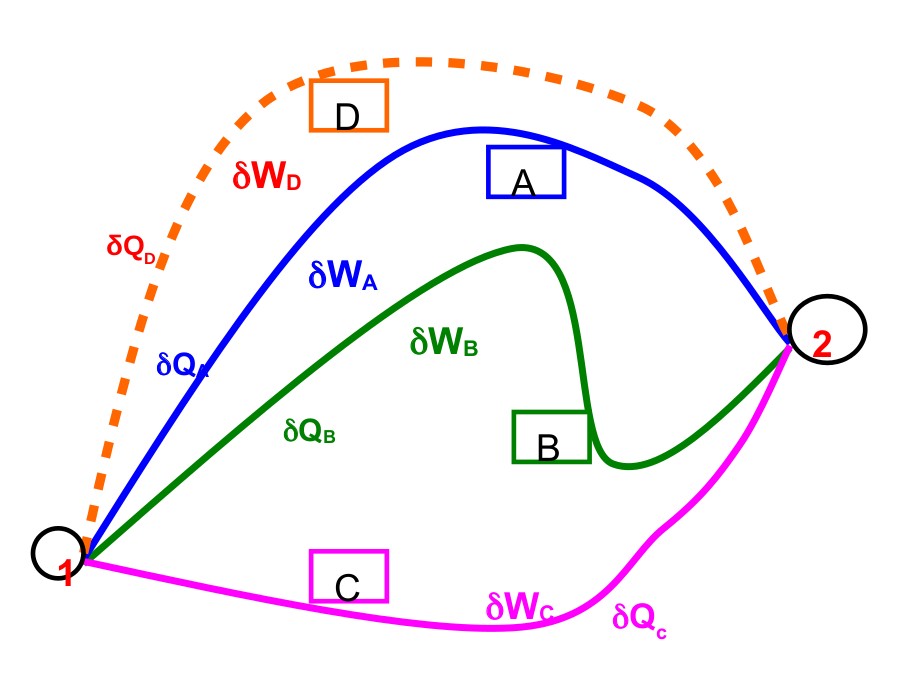
\includegraphics[
            width=0.45\textwidth
        ]   {thermodynamicProcesses.png}

        \label{fig:thermodynamicProcesses}
    \end{figure}

    Nos processos reversíveis, todos os estados que compõe a trajetória do
    processo podem ser identificados, ao passo que nos processos irreversíveis,
    só se consegue identificar o estado inicial e o final, como no processo D,
    representado com linhas pontilhadas na \cref{fig:thermodynamicProcesses}.

    Entretanto, uma discussão mais extensa sobre irreversibilidade será adiada
    até estudarmos a Segunda lei da Termodinâmica.

    Portanto, você já sabe que as interações de energia na fronteira são de
    forma a que:
	%
	\begin{equation}
        \idiff{\ensuremath{\gls{heatTransfer}_{A}}}
        \neq
        \idiff{\ensuremath{\gls{heatTransfer}_{B}}}
        \neq
        \idiff{\ensuremath{\gls{heatTransfer}_{C}}}
        \neq
        \idiff{\ensuremath{\gls{heatTransfer}_{D}}}
    \end{equation}

    e
	%
	\begin{equation}
        \idiff{\ensuremath{\gls{workTransfer}_{A}}}
        \neq
        \idiff{\ensuremath{\gls{workTransfer}_{B}}}
        \neq
        \idiff{\ensuremath{\gls{workTransfer}_{C}}}
        \neq
        \idiff{\ensuremath{\gls{workTransfer}_{D}}}\,.
    \end{equation}

    Observe também que trabalho e calor só existem durante a ocorrência de cada
    processo que leva do estado inicial 1 para o estado final 2, daí a
    afirmação de que calor e trabalho representam formas de energia em trânsito
    através da fronteira do sistema. Na verdade, como já dissemos, a notação
    \enquote{\idiff{}} é comumente utilizada para calor e trabalho em processos
    infinitesimais, ou seja, um infinitésimo separa o estado 1 do estado 2.

    Pois bem, imagine que a temperatura e a pressão referentes ao estado 1
    sejam respectivamente \state{\gls{temperature}}{1} e
    \state{\gls{pressure}}{1} ao passo que a temperatura e a pressão referentes
    ao estado 2 sejam \state{\gls{temperature}}{2} e \state{\gls{pressure}}{2}
    respectivamente. A propósito, ao longo deste trabalho usaremos a notação de
    sobrescrito entre parênteses para denotar o estado e, principalmente no
    caso de misturas, reservaremos o subscrito para denotar o componente. Como
    estes estados 1 e 2 estão infinitesimalmente separados e, de acordo com a
    definição, as propriedades termodinâmicas não dependem  do processo, a
    variação de temperatura e de pressão entre os dois estados será
    \diff{\gls{temperature}} e \diff{\gls{pressure}}. A notação
    \enquote{\diff{}} será reservada para variação infinitesimal de qualquer
    propriedade termodinâmica, pois são diferenciais ordinárias. Você consegue
    notar a diferença entre os símbolos \enquote{\idiff{}} e \enquote{\diff{}}
    que aparecem nestas grandezas infinitesimais?

    Claramente, devido à dependência do processo e a energia em trânsito, não
    tem sentido algum falarmos em \enquote{variação} de calor ou de trabalho,
    ou seja, não existem os calores puntuais \state{\gls{heatTransfer}}{1} ou
    \state{\gls{heatTransfer}}{2} e os trabalhos puntuais
    \state{\gls{workTransfer}}{1} e \state{\gls{workTransfer}}{2}, ao passo que
    é muito natural nos referirmos à variação de temperatura, volume, massa,
    pressão ou de qualquer outra propriedade termodinâmica.

    Se o processo for finito (e não infinitesimal) a notação passa a ser
    \fprocess{heatTransfer}{1}{2}{A} e \fprocess{workTransfer}{1}{2}{A}  para
    trabalho e calor e $\Delta \gls{temperature}$ e $\Delta \gls{pressure}$
    para temperatura, pressão (e, enfim, para qualquer propriedade
    termodinâmica), resultado de integrações como nas equações 0.3 e 0.4.
	%
	\begin{equation} \label{eq:0.3}
        \fprocess{heatTransfer}{1}{2}{A}
        =
        \int\limits_{1}^{2}{%
            \idiff{\gls{heatTransfer}_{A}}
        }
    \end{equation}

    e
	%
	\begin{equation} \label{eq:0.4}
        \fprocess{workTransfer}{1}{2}{A}
        =
        \int\limits_{1}^{2}{%
            \idiff{\gls{workTransfer}_{A}}
        }
    \end{equation}

    A propósito, apenas por convenção, ambos, o calor que entra no sistema e o
    trabalho realizado pelo sistema (que \enquote{sai} do sistema) são
    considerados positivos, enquanto que o calor que sai do sistema e o
    trabalho realizado sobre o sistema (\enquote{entra} no sistema) são ambos
    negativos. A convenção a respeito do calor é praticamente universal, mas
    como já dissemos, preste atenção à do trabalho, pois existe muita
    literatura, principalmente da Química ou da Engenharia Química, que adota a
    convenção contrária a nossa.

    Antes de estudarmos a relação entre as interações na fronteira de um
    sistema e alterações em suas propriedades termodinâmicas, vamos discutir
    com mais cuidado a caracterização do estado como sendo um retrato
    instantâneo de todas as propriedades termodinâmicas do sistema. Por
    enquanto, só conhecemos as propriedades \gls{mass}, \gls{volume},
    \gls{specificVolume}, \gls{temperature}, \gls{pressure} e claramente nem
    todas são independentes (por quê?).

